% !TeX program = xelatex
\documentclass[lang=cn,chinesefont=nofont,a4paper,newtx]{elegantpaper}

\title{Multi-AMR Warehouse Scheduling 灵敏度分析}
\author{运筹学大作业小组}
\date{}

\newcommand{\Cmax}{C_{\max}}
\newcommand{\indicator}{\mathbf{1}}
\newcommand{\thetaop}{\boldsymbol{\theta}}

\usepackage{tikz}
\usetikzlibrary{arrows.meta,positioning}

\setCJKmainfont{Songti SC}
\setCJKsansfont{PingFang SC}
\setCJKmonofont{Hiragino Sans GB}

\graphicspath{{../figures/}}

\begin{document}

\maketitle

\begin{abstract}
本文围绕多 AMR 仓库调度系统的性能退化原因开展灵敏度分析。分析保持与前序调度流程一致，围绕 AMR 数量、任务负荷与瓶颈通道容量三个可解释参数，判断系统性能恶化究竟来自资源不足还是局部拥堵。
\keywords{多 AMR 调度，灵敏度分析，Cmax，拥堵热点，滚动重排}
\end{abstract}

\section{灵敏度分析}
多 AMR 仓库调度的运行效果由资源配置与约束紧性共同决定。本部分围绕多 AMR 仓库调度系统的性能退化原因开展灵敏度分析。在本项目中，仓库拓扑、任务规则和动态事件机制给定后，调度系统的主要可控因素集中在 \textbf{AMR 数量、任务负荷和通道通行能力}。AMR 数量决定可用运输资源，任务负荷决定资源需求强度，通道容量决定局部路网约束。三者均可由工程措施直接改变，并且会同时影响任务分配、车辆排序、路径占用和动态重排结果。

在实际运营中，我们需要知道真正制约系统的资源瓶颈。若 \textbf{增加 AMR} 后完工时间改善明显，扩车具有直接价值；若任务量增加后等待和重排快速上升，说明系统已接近 \textbf{任务负荷边界}；若少数通道长期高占用并引发冲突，说明应优先关注 \textbf{局部通行能力}。灵敏度分析的意义就在于把这些现象拆成可比较的实验结果，支撑后续投入选择。

因此，我们以当前仓库布局、任务集合和动态事件为基准，依次进行 \textbf{基线校验}、\textbf{AMR 数量边际分析}、\textbf{任务负荷边界识别}、\textbf{热点通道容量检验} 和 \textbf{工程干预对比}。最终结论服务于三个直接决策：是否继续扩充 AMR，是否控制单位周期内的任务释放量，是否优先改造瓶颈区域。

\subsection{基线校验与占用热点识别}

进行关键资源敏感度分析之前，我们首先固定当前实例的\textbf{真实调度结果}。基线工况包含当前仓库布局、12 个静态任务、4 台 AMR，以及已注入的动态事件。系统依次完成\textbf{静态排程、冲突修复和动态重排}；同时将轨迹点投影到网格单元，统计\textbf{轨迹占用热点}。关键结果汇总见表~\ref{tab:baseline-summary} 和表~\ref{tab:baseline-hotspots}。

\begin{center}
\begin{minipage}[t]{0.53\linewidth}
\centering
\small
\captionof{table}{基线工况关键结果}
\label{tab:baseline-summary}
\renewcommand{\arraystretch}{1.76}
\begin{tabular}{@{}lll@{}}
\toprule
模块 & 任务 / AMR & $\Cmax$ \\
\midrule
静态排程 & 12 / 4 & 40.840111 \\
冲突修复 & 12 / 4 & 46.596970 \\
动态重排 & 13 / 4 & 61.918082 \\
\bottomrule
\end{tabular}
\renewcommand{\arraystretch}{1}
\end{minipage}
\hfill
\begin{minipage}[t]{0.39\linewidth}
\centering
\small
\captionof{table}{基线轨迹占用热点}
\label{tab:baseline-hotspots}
\begin{tabular}{@{}ccc@{}}
\toprule
热点 & 网格坐标 & 占用次数 \\
\midrule
1 & $(6,4)$ & 166 \\
2 & $(5,4)$ & 152 \\
3 & $(9,1)$ & 95 \\
4 & $(9,2)$ & 84 \\
5 & $(8,2)$ & 77 \\
\bottomrule
\end{tabular}
\end{minipage}
\end{center}

由表~\ref{tab:baseline-summary} 可见，\textbf{冲突修复使 $\Cmax$ 从 40.840111 上升到 46.596970，增幅约 14.1\%}；\textbf{动态重排后 $\Cmax$ 进一步上升到 61.918082，较冲突修复结果增加约 32.9\%}。与此同时，总延期、剩余冲突和硬违规均为 0，说明\textbf{基线排程具有可行性}；变更任务 4 个、新增任务 1 个，则说明\textbf{动态事件已经带来可观的计划扰动}。表~\ref{tab:baseline-hotspots} 显示，$(6,4)$ 与 $(5,4)$ 两个相邻网格占用最高，分别达到 166 次和 152 次；$(9,1)$、$(9,2)$ 和 $(8,2)$ 也形成\textbf{连续的高占用区域}。

为解释完工时间上升背后的空间原因，我将轨迹点投影到\textbf{网格单元} $\Omega_{ab}$，并统计\textbf{占用次数与归一化占用密度}：
\begin{equation}
H_{ab}=\sum_{k=1}^{N}\indicator\{(x_k,y_k)\in\Omega_{ab}\},
\qquad
\rho_{ab}=\frac{H_{ab}}{\sum_{p,q}H_{pq}}.
\end{equation}
对应空间分布见图~\ref{fig:baseline-dashboard}。图~\ref{fig:baseline-dashboard} 集中可视化展现了前文的\textbf{运筹策略与资源占有情况}.

\begin{center}
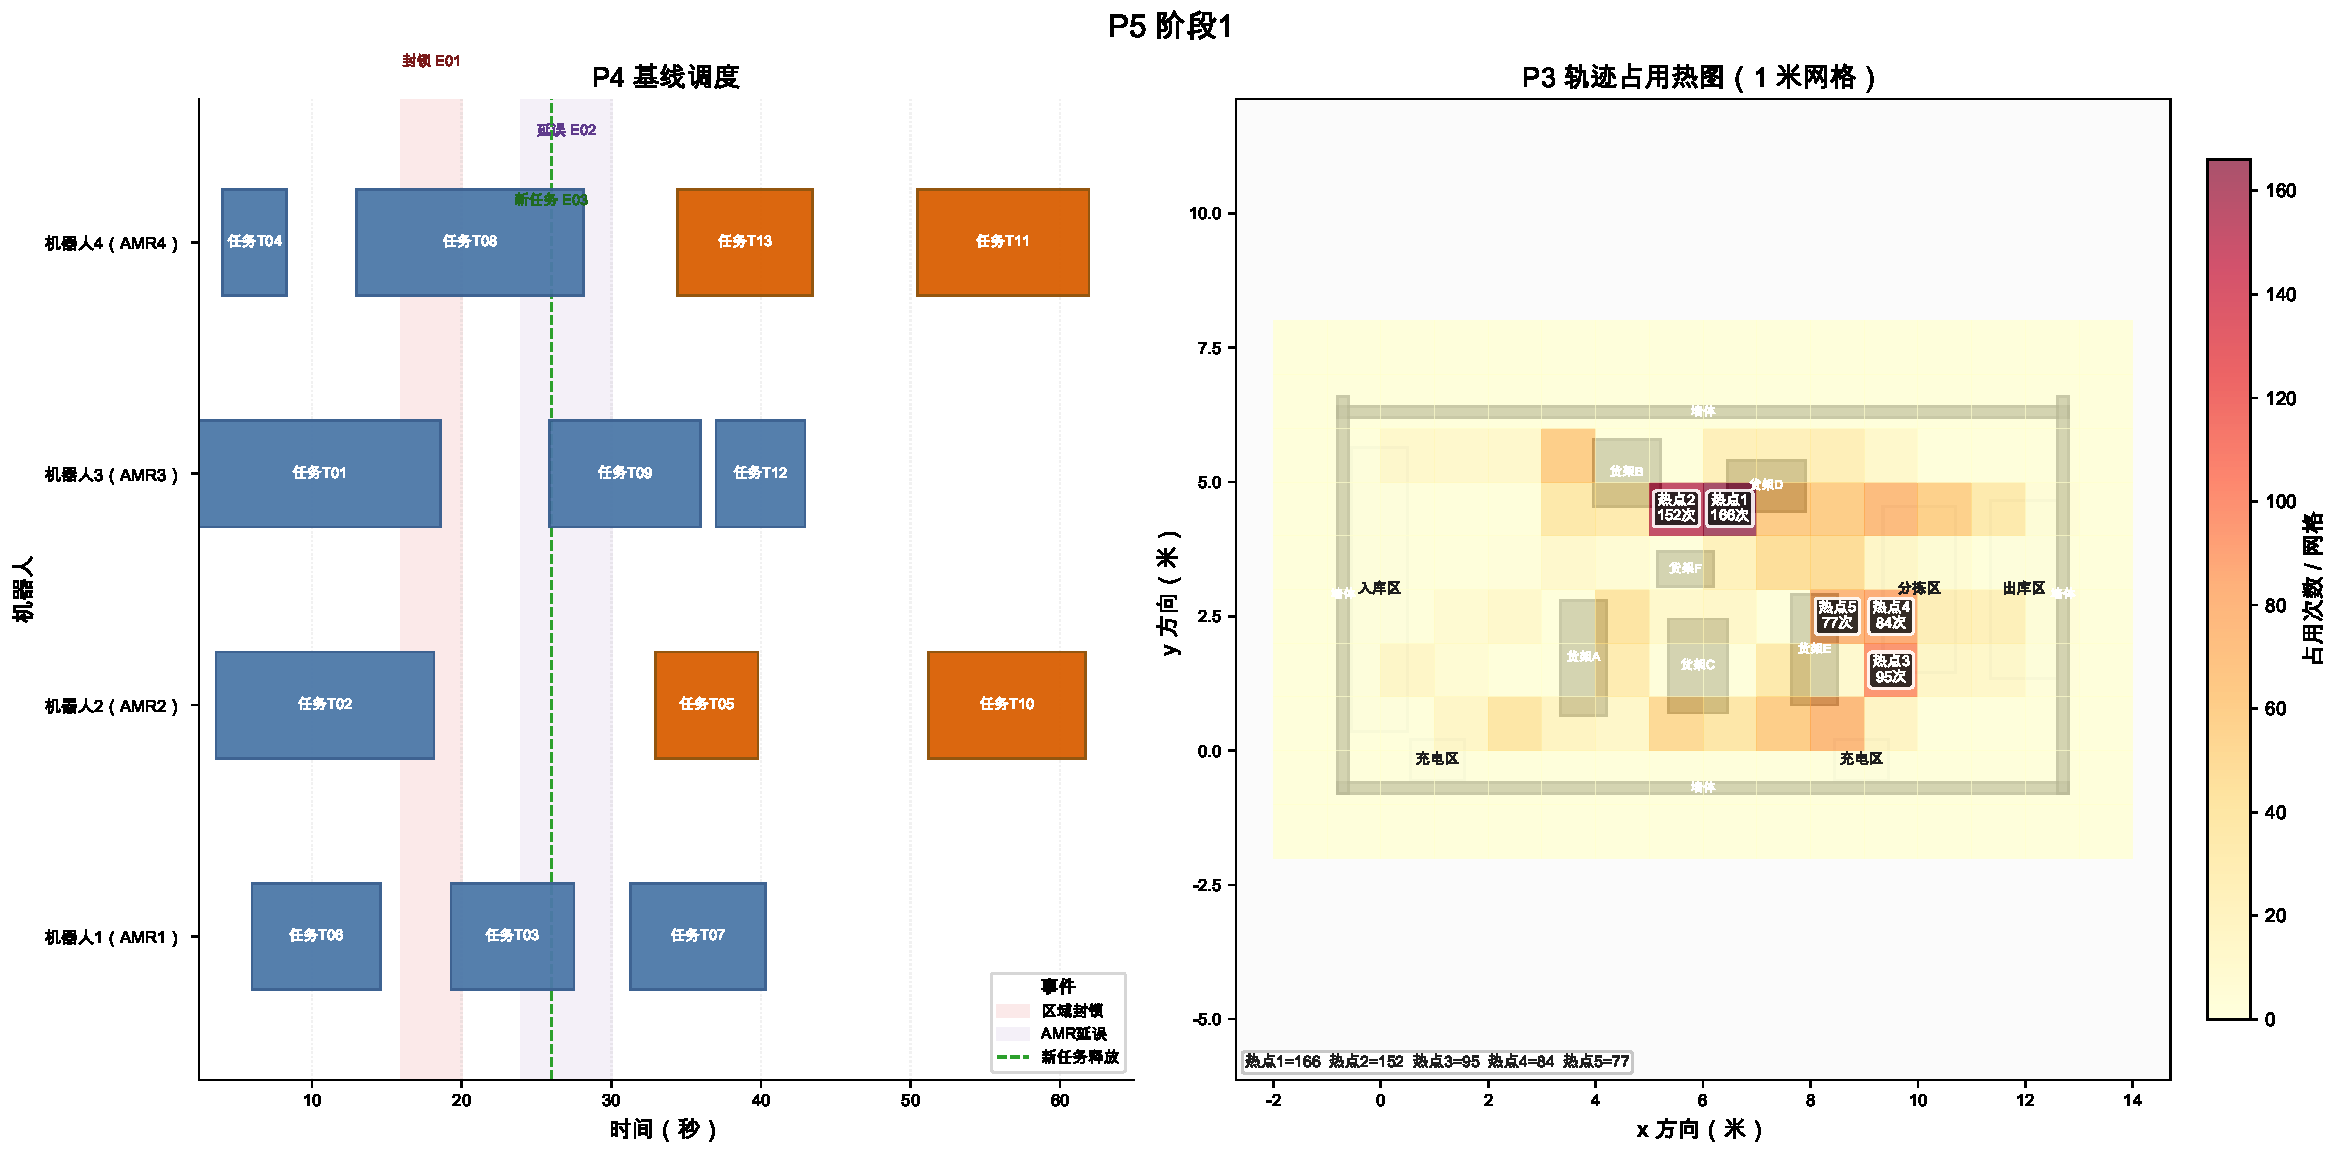
\includegraphics[width=0.94\linewidth]{baseline_dashboard}
\captionof{figure}{基线工况下的重排甘特图与轨迹占用热图}
\label{fig:baseline-dashboard}
\end{center}

综合表~\ref{tab:baseline-summary}、表~\ref{tab:baseline-hotspots} 和图~\ref{fig:baseline-dashboard}，\textbf{当前系统已经满足可行性校验，同时表现出局部拥堵与动态扰动}。敏感度分析因此围绕\textbf{AMR 资源冗余、任务负荷边界和瓶颈通道容量}展开。

\subsection{AMR 数量的资源边际分析}

AMR 数量是仓库调度系统中最直接的\textbf{资源变量}。车辆不足时，任务会在少数 AMR 上串行排队，\textbf{时间窗延期和最大完工时间同时上升}；车辆过多时，继续扩车只能带来\textbf{有限吞吐裕度}。因此，本部分固定仓库布局、12 个任务、时间窗、电量规则和 mixed 路径代价，只改变整数资源参数 $m$，分析 $m$ 的\textbf{边际响应}。

AMR 数量 $m$ 为\textbf{离散整数资源}，局部敏感度采用\textbf{枚举重优化后的前向有限差分}。对任一随 $m$ 变化的性能指标 $G(m)$，定义
\begin{equation}
\Delta^+G(m)=G(m)-G(m+1)\qquad \text{一台 AMR 增量响应}.
\end{equation}
我们以\textbf{运筹调配问题}中最关心的\textbf{最大完工时间}为核心性能指标，并定义
\begin{equation}
\begin{aligned}
\Delta^+\Cmax(m) &= \Cmax(m)-\Cmax(m+1),\\
r_m &= \frac{\Delta^+\Cmax(m)}{\Cmax(m)},\\
\varepsilon_m &= \frac{\Delta^+\Cmax(m)/\Cmax(m)}{1/m}=m\,r_m.
\end{aligned}
\end{equation}
$\Delta^+\Cmax(m)$ 表示完工时间下降量，$r_m$ 表示相对下降比例，$\varepsilon_m$ 表示\textbf{离散弹性近似}。

为判断上述改善是否真正消除\textbf{服务风险}，结合 AMR 调运的项目具体情况构造\textbf{服务状态指标}。设 $\mathcal{J}$ 为任务集合，$\mathcal{K}_m$ 为 AMR 集合，$|\mathcal{K}_m|=m$；参数 $\theta_0$ 表示固定的布局、路径代价、时间窗、服务时间、初始位置和电量规则。给定 $m$ 后，调用主求解流程并记返回方案为 $\hat{\pi}_m$。评价器对 $\hat{\pi}_m$ 进行\textbf{时间和电量仿真}，得到任务完成时刻 $C_j(m)$、任务最晚完成时刻 $\ell_j$、路径缺失次数和电量违规次数。定义
\begin{align}
D_j(m) &= \max\{0,C_j(m)-\ell_j\}, \notag\\
\Cmax(m) &= \max_{j\in\mathcal{J}}C_j(m).
\intertext{$D_j(m)$ 表示任务延期，$\Cmax(m)$ 表示最大完工时间。据此定义服务可行性指标}
S(m) &= \sum_{j\in\mathcal{J}}D_j(m), \notag\\
L(m) &= \sum_{j\in\mathcal{J}}\indicator\{D_j(m)>0\}, \notag\\
M(m) &= N_{\mathrm{trans}}^{\mathrm{miss}}(m)+N_{\mathrm{load}}^{\mathrm{miss}}(m), \notag\\
E(m) &= N_{\mathrm{energy}}^{\mathrm{viol}}(m), \notag\\
Q(m) &= \indicator\{S(m)=0,\ L(m)=0,\ M(m)=0,\ E(m)=0\}.
\end{align}
$S(m)$ 表示总延期，$L(m)$ 表示延期任务数，$M(m)$ 表示路径不可达次数，$E(m)$ 表示电量违规次数，$Q(m)$ 表示\textbf{服务可行性}。
为辅助判断\textbf{资源是否紧张}，记 $A_{\mathrm{act}}(m)$ 为空驶、载货行驶和服务时间之和，并定义
\begin{equation}
\rho(m)=\frac{A_{\mathrm{act}}(m)}{m\,\Cmax(m)}.
\end{equation}
$\rho(m)$ 表示\textbf{平均资源利用率}。

图~\ref{fig:amr-marginal} 同时展示\textbf{资源前沿、有限差分、服务风险和车辆负载}。\textbf{4 台 AMR 是服务风险消除点}；\textbf{5 台以后 $\Cmax$ 仍下降，但边际改善明显减弱}。
\begin{center}
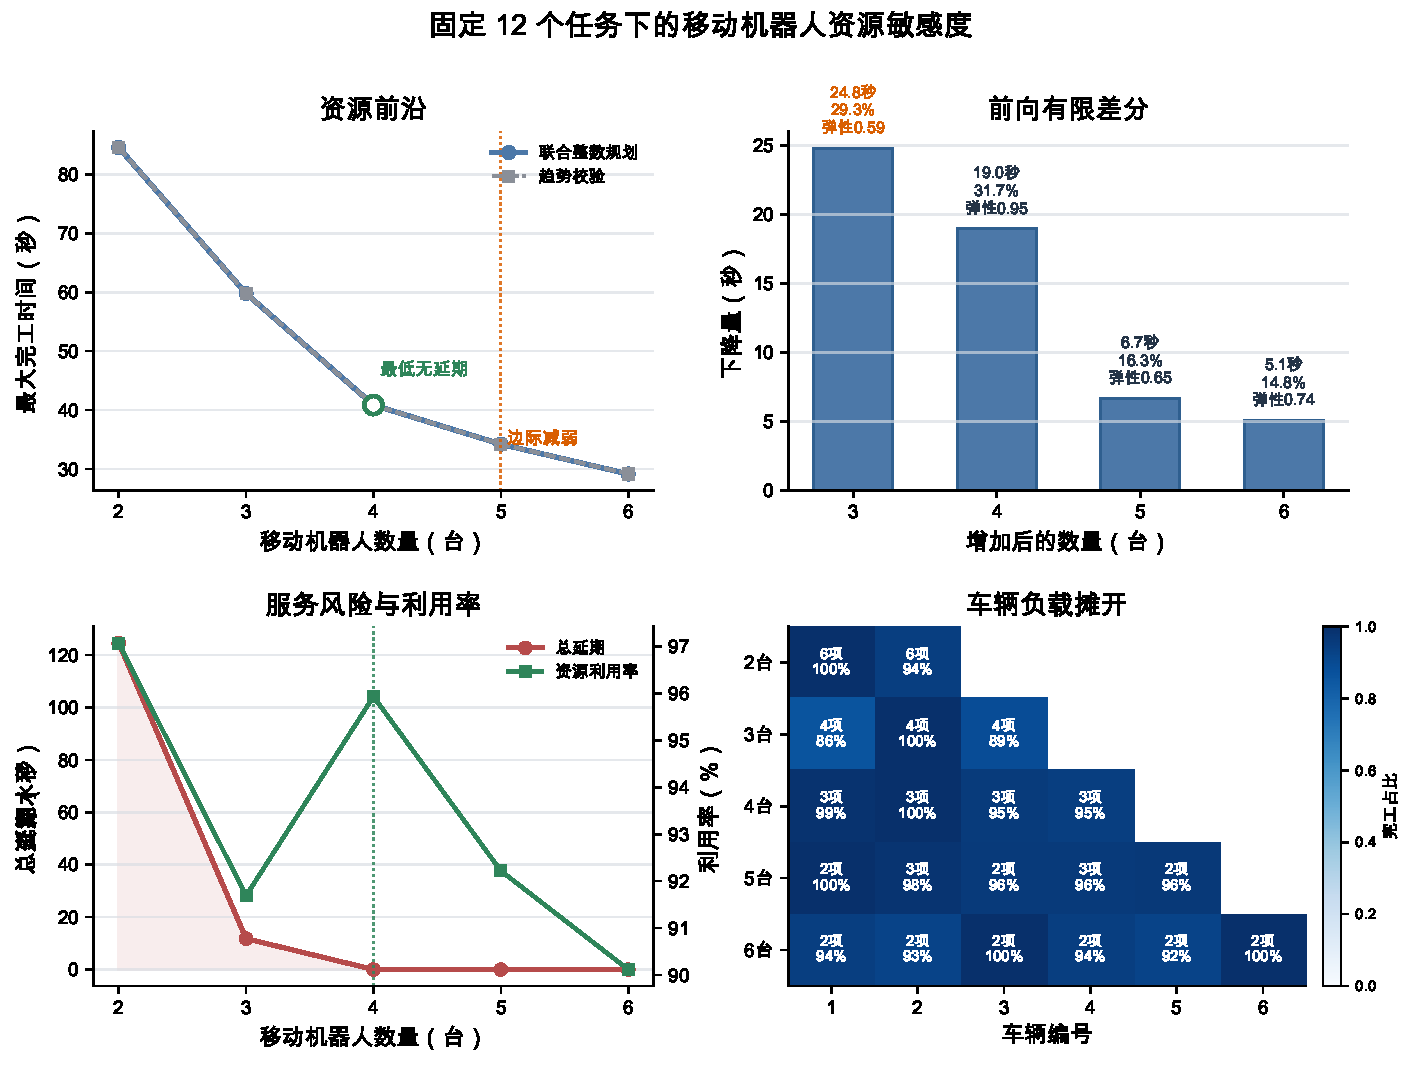
\includegraphics[width=0.95\linewidth]{amr_marginal}
\captionof{figure}{固定任务集下 AMR 数量的资源前沿、前向有限差分、服务风险与车辆负载}
\label{fig:amr-marginal}
\end{center}

\begin{center}
\footnotesize
\begin{minipage}[t]{0.50\linewidth}
\centering
\captionof{table}{AMR 资源前沿}
\label{tab:amr-resource-frontier}
\begin{tabular}{@{}cccccc@{}}
\toprule
$m$ & $\Cmax$ & $S$ & $L$ & $\rho$ & $Q$ \\
\midrule
2 & 84.606 & 124.593 & 4 & 97.08\% & 否 \\
3 & 59.802 & 11.802 & 1 & 91.69\% & 否 \\
4 & 40.840 & 0.000 & 0 & 95.94\% & 是 \\
5 & 34.189 & 0.000 & 0 & 92.22\% & 是 \\
6 & 29.130 & 0.000 & 0 & 90.12\% & 是 \\
\bottomrule
\end{tabular}
\end{minipage}\hfill
\begin{minipage}[t]{0.46\linewidth}
\centering
\captionof{table}{增加一台 AMR 的前向有限差分}
\label{tab:amr-finite-diff}
\begin{tabular*}{\linewidth}{@{\extracolsep{\fill}}ccccc@{}}
\toprule
区间 & $\Delta^+\Cmax$ & $r_m$ & $\varepsilon_m$ & 跨越 \\
\midrule
2--3 & 24.804 & 29.32\% & 0.586 & 否 \\
3--4 & 18.962 & 31.71\% & 0.951 & 是 \\
4--5 & 6.651 & 16.29\% & 0.651 & 否 \\
5--6 & 5.059 & 14.80\% & 0.740 & 否 \\
\bottomrule
\end{tabular*}
\end{minipage}
\end{center}

表~\ref{tab:amr-resource-frontier} 与表~\ref{tab:amr-finite-diff} 表明，\textbf{2 台和 3 台 AMR 均存在服务风险}，\textbf{$m=4$ 时总延期、延期任务数、路径缺失和电量违规同时降为 0，首次达到可行服务状态}。前向有限差分显示，\textbf{3 到 4 台是关键敏感区间}，虽然 $\Delta^+\Cmax$ 小于 2 到 3 台，但完成\textbf{服务阈值跨越}，且\textbf{离散弹性达到 0.951}。\textbf{4 台以后继续扩车只降低 $\Cmax$，不再改变服务可行性，因此 4 台 AMR 是当前算例的服务阈值，5 台可作为高裕度工况参考。}

\subsection{任务负荷与系统容量边界}

在 AMR 数量固定后，进一步需要回答的是当前系统在一个业务时域内最多能稳定处理多少任务。这里不复用 P2 已有的任务密度敏感度实验结果，而是在 P5 中单独构造\textbf{嵌套任务池并逐点重优化}；P2 仅作为单个工况的\textbf{任务分配与排序求解器}被调用。这样可以保证任务负荷参数 $n$ 的变化具有\textbf{严格可比性}，并且\textbf{容量边界来自同一套业务判定规则}。

本阶段固定仓库布局、mixed 路径库和 4 台 AMR。业务时域取
\begin{equation}
H=55\text{ s},
\end{equation}
其来源是基线静态任务批次的最大最晚完成时刻，表示当前任务波次的\textbf{服务承诺时域}。对每个随机种子 $s$，P5 先生成最大任务池 $T_s(N)$，然后只取前缀形成不同规模的任务集合：
\begin{equation}
T_s(n)=\{j_1,\ldots,j_n\},\qquad T_s(n)\subset T_s(n+1).
\end{equation}
因此，\textbf{$n$ 增大时只是在同一个任务池上增加新任务，而不是更换另一批任务样本}。对每个 $(s,n)$，调用同一 P2 静态优化入口得到完工时间 $C_{\max,s}(n)$、总延期、路径缺失和电量违规。\textbf{容量判定采用保守的 all-seeds 规则}：
\begin{equation}
I_s(n)=\indicator\{C_{\max,s}(n)\le H,\ \text{feasible}_s(n)=1\},
\qquad
n_{\mathrm{capacity}}=\max\{n:\prod_s I_s(n)=1\}.
\end{equation}

为刻画任务负荷的局部响应，采用\textbf{离散重优化后的前向有限差分}。令
\(\widetilde{C}_{\max}(n)\) 表示多种子中位数完工时间，并定义
\begin{equation}
\Delta_n \Cmax=\widetilde{C}_{\max}(n+1)-\widetilde{C}_{\max}(n),
\qquad
e_n=\frac{n}{\widetilde{C}_{\max}(n)}\Delta_n \Cmax.
\end{equation}
$\Delta_n\Cmax$ 表示增加一个任务带来的\textbf{边际完工时间增量}，$e_n$ 是归一化后的\textbf{任务负荷弹性}。该指标来自\textbf{离散工况重优化结果}，不使用插值或平滑曲线替代实际求解点。

\begin{center}
\small
\captionof{table}{任务负荷容量边界附近的离散扫描结果}
\label{tab:task-capacity-frontier}
\begin{tabular}{@{}cccccc@{}}
\toprule
$n$ & $\min \Cmax$ & $\mathrm{median}\ \Cmax$ & $\max \Cmax$ & $\Delta_n\Cmax$ & all-seeds \\
\midrule
12 & 40.840 & 40.840 & 40.840 & 4.884 & 是 \\
13 & 44.927 & 45.724 & 45.724 & 4.202 & 是 \\
14 & 49.840 & 49.926 & 50.465 & 6.142 & 是 \\
15 & 51.537 & 56.068 & 58.345 & 3.654 & 否 \\
16 & 55.512 & 59.723 & 66.559 & 6.959 & 否 \\
\bottomrule
\end{tabular}
\end{center}

\begin{center}
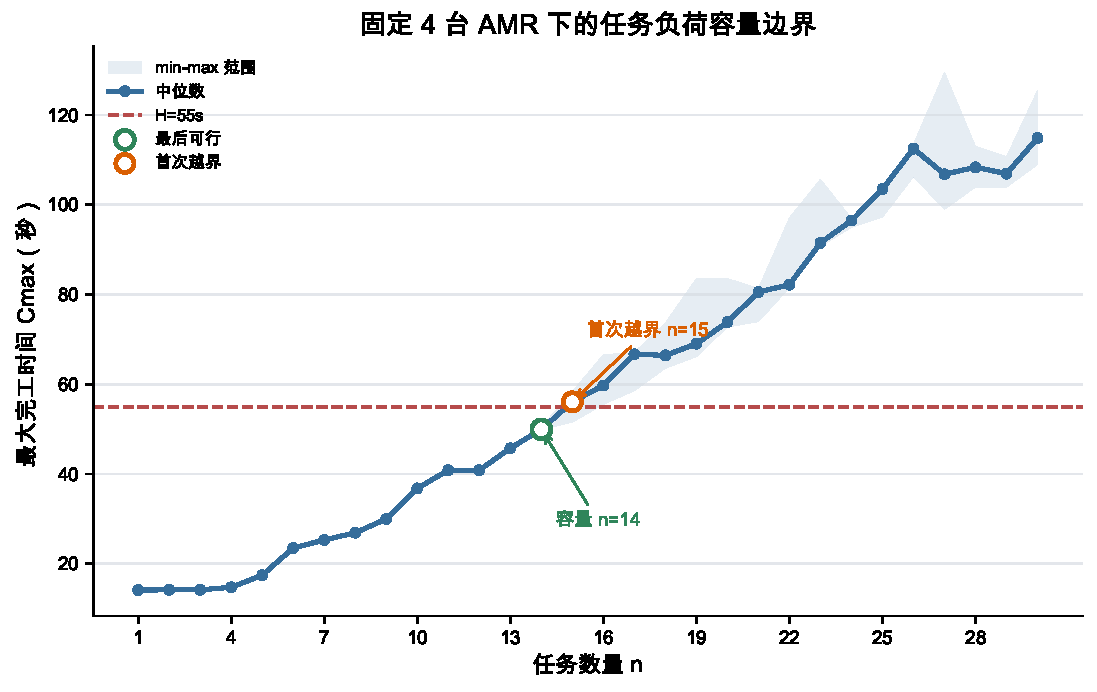
\includegraphics[width=0.74\linewidth]{task_capacity}
\captionof{figure}{固定 4 台 AMR 下的任务负荷容量边界}
\label{fig:task-capacity}
\end{center}

图~\ref{fig:task-capacity} 给出 $n\mapsto \Cmax(n)$ 的\textbf{容量边界曲线}。蓝线为多种子中位数，浅色带表示 min--max 范围，红色虚线为统一业务时域 $H$。由表~\ref{tab:task-capacity-frontier} 可见，\textbf{$n=14$ 时三个种子均满足 $C_{\max,s}(n)\le 55$ 且无硬约束违规}；\textbf{$n=15$ 时中位数已经达到 56.068222，且只有 1 个种子仍满足时域约束}。因此，在固定 4 台 AMR 和 mixed 路径库下，本轮离散重优化得到的\textbf{保守容量边界}为
\begin{equation}
n_{\mathrm{capacity}}=14,\qquad n_{\mathrm{cross}}=15.
\end{equation}
需要注意的是，\textbf{$\Delta_n\Cmax$ 是每个负荷水平重新优化后的离散响应}；个别高负荷点可能因任务组合和整数重优化结果变化出现\textbf{非单调有限差分}，因此不对曲线做单调化处理，也不使用插值曲线替代离散求解结果。

\subsection{瓶颈空间簇与容量影子价值}

任务负荷容量边界给出了系统最多能承受的任务规模，但仍需进一步定位限制调度性能的空间资源。

\subsubsection{边界工况与离散影子价值}

本节选择前文任务负荷与系统容量边界中接近容量边界且仍满足业务时域的工况，即 $n_{\mathrm{capacity}}=14$、方法为 M2 的种子 1 工况，并在该工况上重新展开 P3 时空冲突修复。\textbf{我们把仓库局部通道视为有限容量资源，计算其容量单位放松后的边际价值。}

设 $C$ 为空间网格连通簇，$N_{C,t}$ 为时间桶 $t$ 中占用簇 $C$ 的 AMR 数。基线容量约束抽象为
\begin{equation}
N_{C,t}\leq q_C,\qquad q_C=1.
\end{equation}
这里的 \textbf{$q_C$ 是局部能同时通过的 AMR 数量}。\textbf{执行 $q_C:1\rightarrow 2$ 可以解释为通道拓宽、设置会车区、调整局部交通规则或增加分拣口前缓冲区。}由于当前 P2 的 MILP 没有显式建立边容量约束，本部分对候选空间簇逐一放松容量并重跑 P3 冲突修复优化，得到\textbf{离散影子价值}
\begin{equation}
\pi_C^{J}=J^{\mathrm{base}}-J^{+1}(C),\qquad
\pi_C^{T}=\Cmax^{\mathrm{base}}-\Cmax^{+1}(C),
\end{equation}
其中 P3 修复目标为
\begin{equation}
J=100D_{\mathrm{sum}}+5\Cmax+W+2R+20S+20W_0.
\end{equation}
$D_{\mathrm{sum}}$ 为总延期，$W$ 为冲突修复插入等待，$R$ 为换路次数，$S$ 为同车换序次数，$W_0$ 为初始等待。$\pi_C^J$ 和 $\pi_C^T$ 分别表示簇容量增加 1 后目标函数和最大完工时间的真实改善量；\textbf{最终瓶颈排序以重优化后的有限差分为准，而不是以经过次数或热图颜色为准。}

\begin{center}
\small
\resizebox{0.98\linewidth}{!}{%
\begin{tikzpicture}[
    font=\small,
    analysisstep/.style={
        draw=blue!28!black,
        fill=blue!4,
        rounded corners=2pt,
        line width=0.55pt,
        minimum height=1.18cm,
        text width=3.25cm,
        align=center,
        inner sep=5pt,
        text=black!88
    },
    decisionsstep/.style={
        draw=teal!24!black,
        fill=teal!3,
        rounded corners=2pt,
        line width=0.55pt,
        minimum height=1.18cm,
        text width=3.25cm,
        align=center,
        inner sep=5pt,
        text=black!88
    },
    arrow/.style={-{Stealth[length=2.15mm]}, line width=0.55pt, draw=black!45},
    node distance=0.72cm and 0.92cm
]
\node[analysisstep] (base) {\textbf{1 基线工况}\\边界任务规模\\记录 $\Cmax^{\mathrm{base}},J^{\mathrm{base}},W^{\mathrm{base}}$};
\node[analysisstep, right=of base] (score) {\textbf{2 时空投影}\\轨迹映射到网格--时间桶\\计算 $s(c)$};
\node[analysisstep, right=of score] (cluster) {\textbf{3 候选簇}\\连通合并\\保留冲突/等待信号};
\node[decisionsstep, below=of cluster] (relax) {\textbf{4 容量放松}\\逐簇执行 $q_C\leftarrow q_C+1$\\重跑 P3 修复};
\node[decisionsstep, left=of relax] (value) {\textbf{5 影子价值}\\计算 $\pi_C^J,\pi_C^T$\\按 $\Delta\Cmax$ 排序};
\node[decisionsstep, left=of value] (decision) {\textbf{6 工程判读}\\识别主瓶颈\\给出布局/规则改造};
\draw[arrow] (base) -- (score);
\draw[arrow] (score) -- (cluster);
\draw[arrow] (cluster) -- (relax);
\draw[arrow] (relax) -- (value);
\draw[arrow] (value) -- (decision);
\end{tikzpicture}}
\captionof{figure}{瓶颈空间簇容量敏感度分析流程}
\label{fig:stage4-sensitivity-flow}
\end{center}

\subsubsection{前置筛选}
我们对候选簇进行空间统计。轨迹点按 $1\mathrm{m}\times 1\mathrm{m}$ 网格和 $1\mathrm{s}$ 时间桶投影，并对同一 AMR 在同一时间桶内的重复采样去重。对每个网格 $c$ 计算占用、冲突修复事件、冲突等待和延期压力的标准化分量：
\begin{equation}
s(c)=0.25z(\mathrm{occ}_c)+0.30z(\mathrm{conf}_c)+0.30z(\mathrm{wait}_c)+0.15z(\mathrm{delay}_c).
\end{equation}
相邻高分网格合并成连通簇后，只对含有冲突或等待信号的簇做容量放松重求。\textbf{若一个区域只是经过次数高，但容量放松后 $\pi_C^J$ 近似为 0，则只能称为高流量区，不能作为主瓶颈。}

本工况中，轨迹、冲突、等待和延期信号共覆盖 56 个网格，其中 15 个网格的综合筛选分数为正。采用正分数网格的 70\% 分位数作为阈值，得到 $s(c)\geq 1.731118$ 的高压力网格；再要求该网格必须含有冲突事件或等待信号，最终保留 5 个候选网格。由于这 5 个网格之间不相邻，连通合并后仍为 5 个单元簇，因此它们是由数据自动筛出的候选集，而不是人工指定的固定数量。\textbf{为避免漏检，又对路径库中其余 15 个未纳入网格执行同样的容量 $+1$ 重优化，结果它们的 $\Delta \Cmax$ 均为 0，说明当前主瓶颈没有被前面的筛选遗漏到更强的同类网格。}

\subsubsection{容量放松重优化}

\begin{center}
\small
\captionof{table}{候选瓶颈簇的容量放松有限差分}
\label{tab:bottleneck-capacity-test}
\begin{tabular}{@{}cccccccc@{}}
\toprule
簇 & 位置 & 最近设施 & 筛选分数 & $\Cmax^{\mathrm{base}}$ & $\Cmax^{+1}$ & $\Delta\Cmax$ & $\Delta W$ \\
\midrule
C03 & $(9,2)$ & RACK\_E / Z\_SORT & 1.776 & 83.870 & 69.142 & 14.728 & 49.0 \\
C02 & $(6,4)$ & RACK\_D / Z\_SORT & 3.220 & 83.870 & 80.950 & 2.920 & 32.0 \\
C04 & $(11,4)$ & WALL\_RIGHT / Z\_OUT & 2.416 & 83.870 & 83.870 & 0.000 & 0.0 \\
C05 & $(12,3)$ & WALL\_RIGHT / Z\_OUT & 2.290 & 83.870 & 83.870 & 0.000 & 0.0 \\
C01 & $(6,2)$ & RACK\_C / Z\_SORT & 2.319 & 83.870 & 83.870 & 0.000 & 0.0 \\
\bottomrule
\end{tabular}
\end{center}

\begin{center}
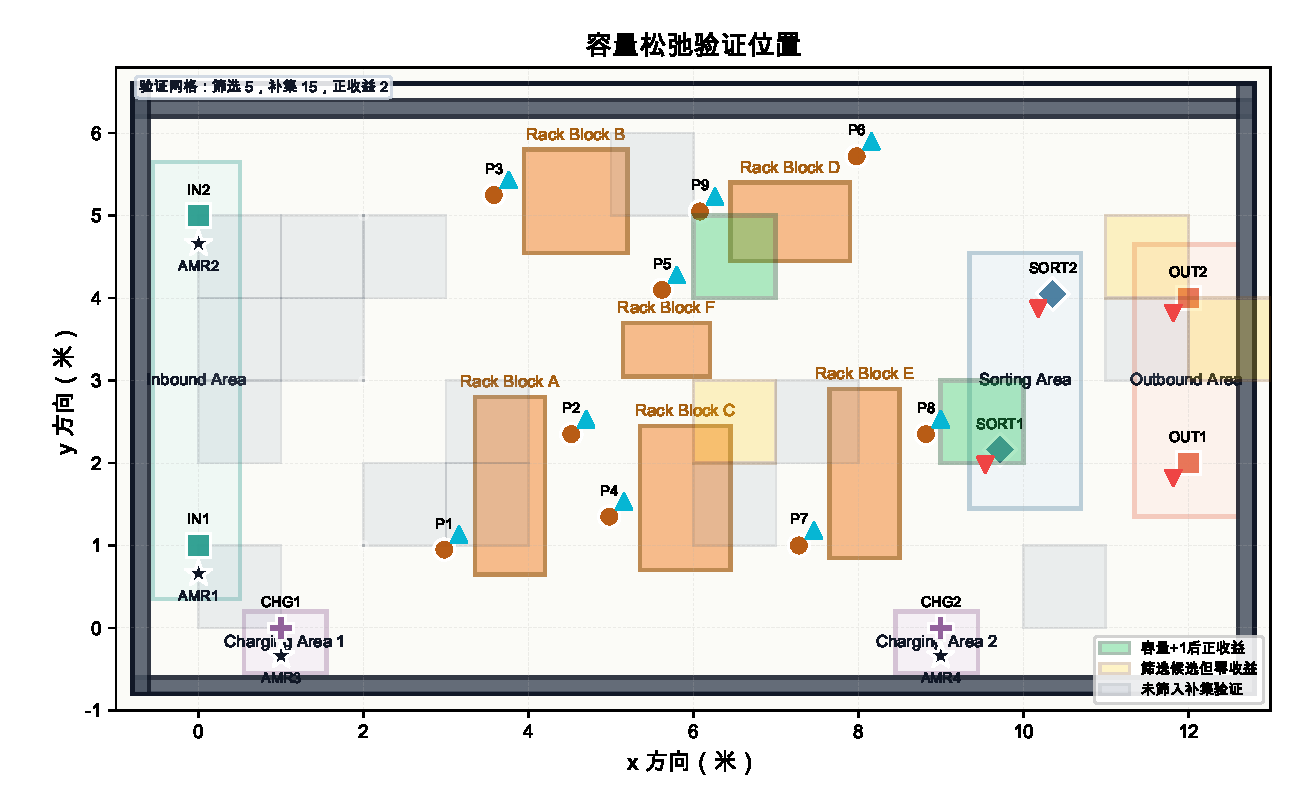
\includegraphics[width=0.95\linewidth]{stage4_bottleneck_cluster}
\captionof{figure}{瓶颈空间簇容量松弛验证位置}
\label{fig:stage4-bottleneck-cluster}
\end{center}

表~\ref{tab:bottleneck-capacity-test} 给出了筛选候选的容量放松结果，图~\ref{fig:stage4-bottleneck-cluster} 展示所有验证位置；路径库补集的 15 个未纳入网格在附加验证中全部得到 $\Delta \Cmax=0$。基线 P3 修复后 $\Cmax=83.869555$，冲突修复等待为 93.0 秒，目标函数为 17263.345675。对 5 个候选空间簇逐一执行容量 $+1$ 并重跑 P3 后，\textbf{C03 的边际改善最大：$\Cmax$ 降至 69.141718，减少 14.727837 秒；冲突等待从 93.0 秒降至 44.0 秒，减少 49.0 秒；目标函数下降 10364.363885。}C02 排名第二，仍有 2.919667 秒的 $\Delta \Cmax$ 和 32.0 秒的等待改善。C04、C05 与 C01 的 $\Delta \Cmax$ 均为 0，其中 C01 甚至出现目标函数轻微上升，说明其容量放松并未缓解当前主要拥堵结构。

\subsubsection{瓶颈排序与工程含义}

因此，\textbf{C03 是当前边界工况下的主导空间瓶颈，位置在 $(9,2)$，对应 RACK\_E 与 Z\_SORT 的汇入带。}这个结论来自容量松弛后的离散影子价值：它同时在 $\Cmax$、总等待和目标函数三个层面都给出最大的边际收益。\textbf{工程上，优先改造 C03 所在通道最有意义，具体措施包括扩大 RACK\_E 附近通道会车能力、在分拣区前设置短缓冲区、限制对向穿越，或将进入 Z\_SORT 的任务释放节奏做错峰控制。}C02 可作为次级改造点继续评估，而 C04、C05 与 C01 更适合保留监测而不是立即扩容。

\subsection{Morris 与 Sobol 全局敏感度筛选}

本阶段将 AMR 数量、任务量和瓶颈簇容量作为同一组\textbf{全局敏感度分析}因素：$Y=f(\theta)=\Cmax(\theta),\theta=(m,n,q_C),$
其中 $m\in\{3,4,5,6\}$，$n\in\{12,13,14,15\}$，$q_C\in\{1,2,3\}$。瓶颈簇 $q_C$ 自动取瓶颈空间簇与容量影子价值分析中排名第一的 C03。所有样本均运行真实前文运筹规划算法调度链路，连续设计点 $x_i\in[0,1]$ 仅用于抽样，实际求解前按
$
\mathcal{M}_i(x_i)=\ell_{i,r_i},
r_i=1+\min\{L_i-1,\max\{0,\mathrm{round}((L_i-1)x_i)\}\}
$
映射到离散水平 $\mathcal{L}_i=(\ell_{i,1},\ldots,\ell_{i,L_i})$，因此响应为 $Y=f(\mathcal{M}(x))$。

\subsubsection{Morris 基本效应筛选}

Morris 方法用\textbf{有限差分基本效应}筛选主导因素。设归一化空间划分为 $p$ 个水平，本实验 $p=4$，步长、第 $r$ 条轨迹上因素 $i$ 的基本效应、对 $R$ 条轨迹汇总定义如下
\[
\Delta=\frac{p}{2(p-1)}=\frac{2}{3}.
\]

\[
EE_i^{(r)}
=\frac{f(\mathcal{M}(x^{(r)}+\Delta e_i))-f(\mathcal{M}(x^{(r)}))}{\Delta}.
\]

\[
\mu_i^\star=\frac{1}{R}\sum_{r=1}^{R}|EE_i^{(r)}|,\qquad
\sigma_i=\sqrt{\frac{1}{R-1}\sum_{r=1}^{R}\left(EE_i^{(r)}-\bar{EE}_i\right)^2}.
\]
其中 $\mu_i^\star$ 表示全局影响强度，$\sigma_i$ 表示影响随背景工况变化的幅度；$\sigma_i$ 较大通常意味着\textbf{非线性效应}或\textbf{交互效应}。

\begin{center}
\small
\captionof{table}{Morris 全局筛选结果}
\label{tab:stage5-morris}
\begin{tabular}{@{}lccc@{}}
\toprule
因素 & $\mu^\star$ & $\sigma$ & $\mu^\star$ 置信宽度 \\
\midrule
$m$ & 30.711 & 10.943 & 6.490 \\
$n$ & 12.318 & 11.580 & 5.310 \\
$q_C$ & 1.875 & 3.841 & 1.971 \\
\bottomrule
\end{tabular}
\end{center}

表~\ref{tab:stage5-morris} 显示，$m$ 的 $\mu^\star=30.711$ 秒，明显高于 $n$ 和 $q_C$；$n$ 的 $\sigma=11.580$ 秒接近 $m$，说明任务量效应强烈依赖车队规模和拥堵背景。\textbf{从 Morris 筛选看，增加 AMR 数量是当前工况下最直接的资源配置杠杆，任务量是次级压力源，单独提高 C03 局部容量的全局收益有限。}

\subsubsection{Sobol 方差分解验证}

Sobol 方法从\textbf{方差分解}度量因素贡献。令 $X=(X_1,\ldots,X_D)$ 且 $D=3$，若 $Y=f(\mathcal{M}(X))$ 平方可积，则
\[
f(X)=f_0+\sum_i f_i(X_i)+\sum_{i<j}f_{ij}(X_i,X_j)+\cdots,\qquad
V=\mathrm{Var}(Y)=\sum_iV_i+\sum_{i<j}V_{ij}+\cdots.
\]
一阶效应和总效应定义为
\[
S_i=\frac{\mathrm{Var}_{X_i}\left(\mathbb{E}_{X_{\sim i}}[Y\mid X_i]\right)}{\mathrm{Var}(Y)},\qquad
S_{T_i}=1-\frac{\mathrm{Var}_{X_{\sim i}}\left(\mathbb{E}_{X_i}[Y\mid X_{\sim i}]\right)}{\mathrm{Var}(Y)}.
\]
$S_i$ 表示因素 $i$ 的独立方差贡献，$S_{T_i}$ 表示包含全部高阶交互后的总贡献。本实验采用 Saltelli/Sobol 设计，$N=64,D=3$，样本规模为 $N(2D+2)=512$。构造 $A,B,A_B^{(i)}$ 后，典型估计量为
\[
\widehat{S_i}=
\frac{\frac{1}{N}\sum_{k=1}^Ny_B^{(k)}(y_{A_B^{(i)}}^{(k)}-y_A^{(k)})}{\widehat V},\qquad
\widehat{S_{T_i}}=
\frac{\frac{1}{2N}\sum_{k=1}^N(y_A^{(k)}-y_{A_B^{(i)}}^{(k)})^2}{\widehat V}.
\]

\begin{center}
\small
\captionof{table}{Sobol 方差分解结果}
\label{tab:stage5-sobol}
\begin{tabular}{@{}lcccc@{}}
\toprule
因素 & $S_1$ & $S_1$ 置信宽度 & $S_T$ & $S_T$ 置信宽度 \\
\midrule
$m$ & 0.752 & 0.343 & 0.880 & 0.362 \\
$n$ & 0.276 & 0.215 & 0.350 & 0.132 \\
$q_C$ & -0.031 & 0.088 & 0.031 & 0.031 \\
\bottomrule
\end{tabular}
\end{center}

\begin{center}
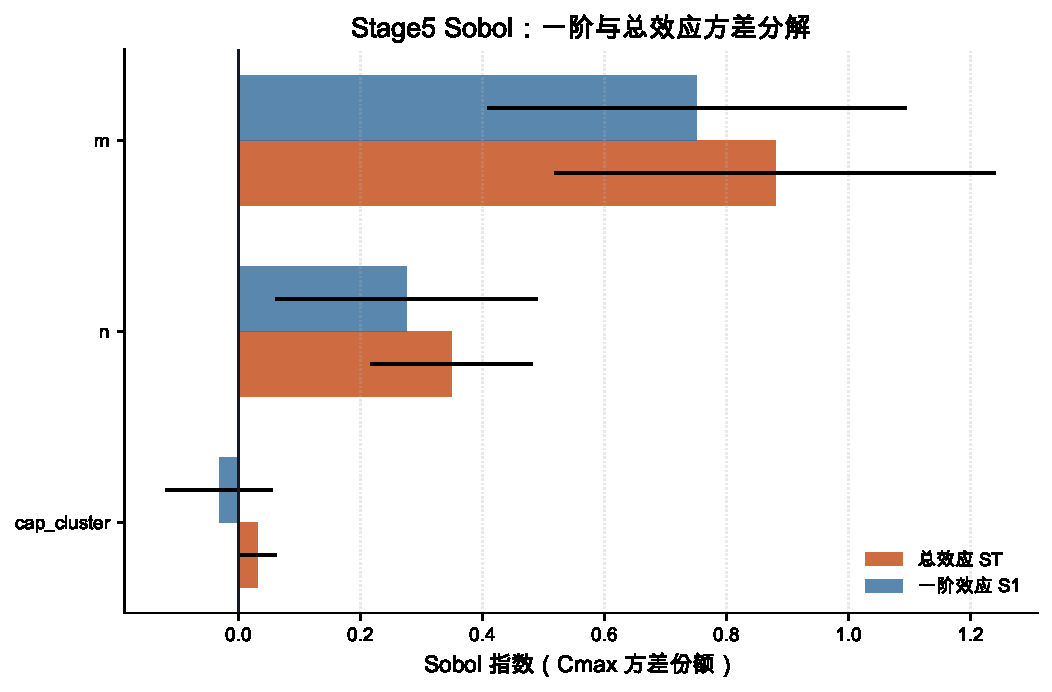
\includegraphics[width=0.6\linewidth]{stage5_sobol}
\captionof{figure}{Sobol 一阶效应与总效应}
\label{fig:stage5-sobol}
\end{center}

表~\ref{tab:stage5-sobol} 和图~\ref{fig:stage5-sobol} 显示，$m$ 的 $S_T=0.880$，显著高于 $n$ 的 0.350 和 $q_C$ 的 0.031。$q_C$ 的 $S_1$ 轻微为负属于有限样本 Monte Carlo 估计误差，不代表容量放松有负贡献；结合其总效应接近 0，可认为 C03 容量在本全局参数域内解释力很弱。\textbf{Sobol 验证了 Morris 排序，$m$ 是主导因素，$n$ 是次级因素，$q_C$ 只适合做局部瓶颈修复。}

\textbf{故名感度分析对仓库管理员的干预优先级作出指导，即优先评估 AMR 数量扩容和任务负荷边界，再对 C03 做针对性容量放松；局部容量放松不能替代全局资源配置。}


\end{document}
